Given the huge transformation that the entire Bitcoin mining activity faced, as analyzed in the previous section, a clarification about two opposite approaches that characterized mining operations since its beginning is needed. In this section the aim is to clarify the operational differences between the so called \textbf{Solo mining} and \textbf{Pooled mining}, focusing on their relative pros and cons.

\subsubsection{Solo mining}
In Solo mining, the miner relies solely on its own computational power to compete against the entire network in the race to find a valid block. In this process the hashes are calculated individually, in order to find a valid block whose reward will be \textbf{paid entirely to the miner} in ownership of the hashing power. This is obtained by explicitly put the miner Bitcoin address into the coinbase output script, when preparing the block template to mine on.
In this case, the miner needs to run a local Bitcoin full-node, to get transactions to validate from, in addiction to the other fields needed to build the block header.\\
However, considering a certain network difficulty defined as \textit{D}, <<Block finding when mining solo with a constant hashrate \textit{h} is a Poisson process with $\frac{h}{2^{32}\cdot D}$ as the rate parameter. We said that mining for time \textit{t} results in $\frac{ht}{2^{32}\cdot D}$ blocks on average.>>\cite{bitcoinpooledmining} As described in the last section, Bitcoin mining became a very competitive field, and since its first years (2011-2013) it definitely started to transform more and more into an industrial activity. Since those years, miners had to start considering many factors during their business activity, such as the intrinsic variance of valid blocks finding during Solo mining. As the Bitcoin network has grown, the mining difficulty has increased significantly. This means that the chances of an individual miner successfully mining a block and earning rewards have diminished considerably. For this reason, since the first years of Bitcoin mining activity, the concept of Pooled mining started to become increasingly popular.

\subsubsection{Pooled mining}
In the current highly competitive mining landscape, solo miners operating alone, face significant challenges. The probability of solo miners successfully finding a block to pay their electricity and hardware expenses has become so low that it constitutes a very risky behaviour. To counter these odds, miners have resulted to collaborating and forming mining pools, systems used to combine their hashing power and sharing the resulting rewards among a large number of participants.\\
Mining pools coordinate thousands of miners, efficiently splitting the nonce search-space and assigning them to individual miners. The individual miners configure their mining equipment to connect to a pool server, and communicate a Bitcoin address to the pool, which is used to receive their share of the rewards. Their mining hardware remains connected to the pool server while mining, synchronizing their efforts with the other miners. In this case, candidate block are built to pay the reward to a pool Bitcoin address, differently from the Solo mining approach. At regular intervals, the pool server initiates payments to the Bitcoin addresses of participating miners once they have accumulated a specific threshold of rewards. The main business model of the pool operators is typically a percentage fee which is cut off from the rewards collected by miners.
To understand how the pool collects the work done by individual miners, the concept of \textbf{\textit{share}} has to be explained.
\begin{wrapfigure}{r}{0.7\textwidth}
\centering
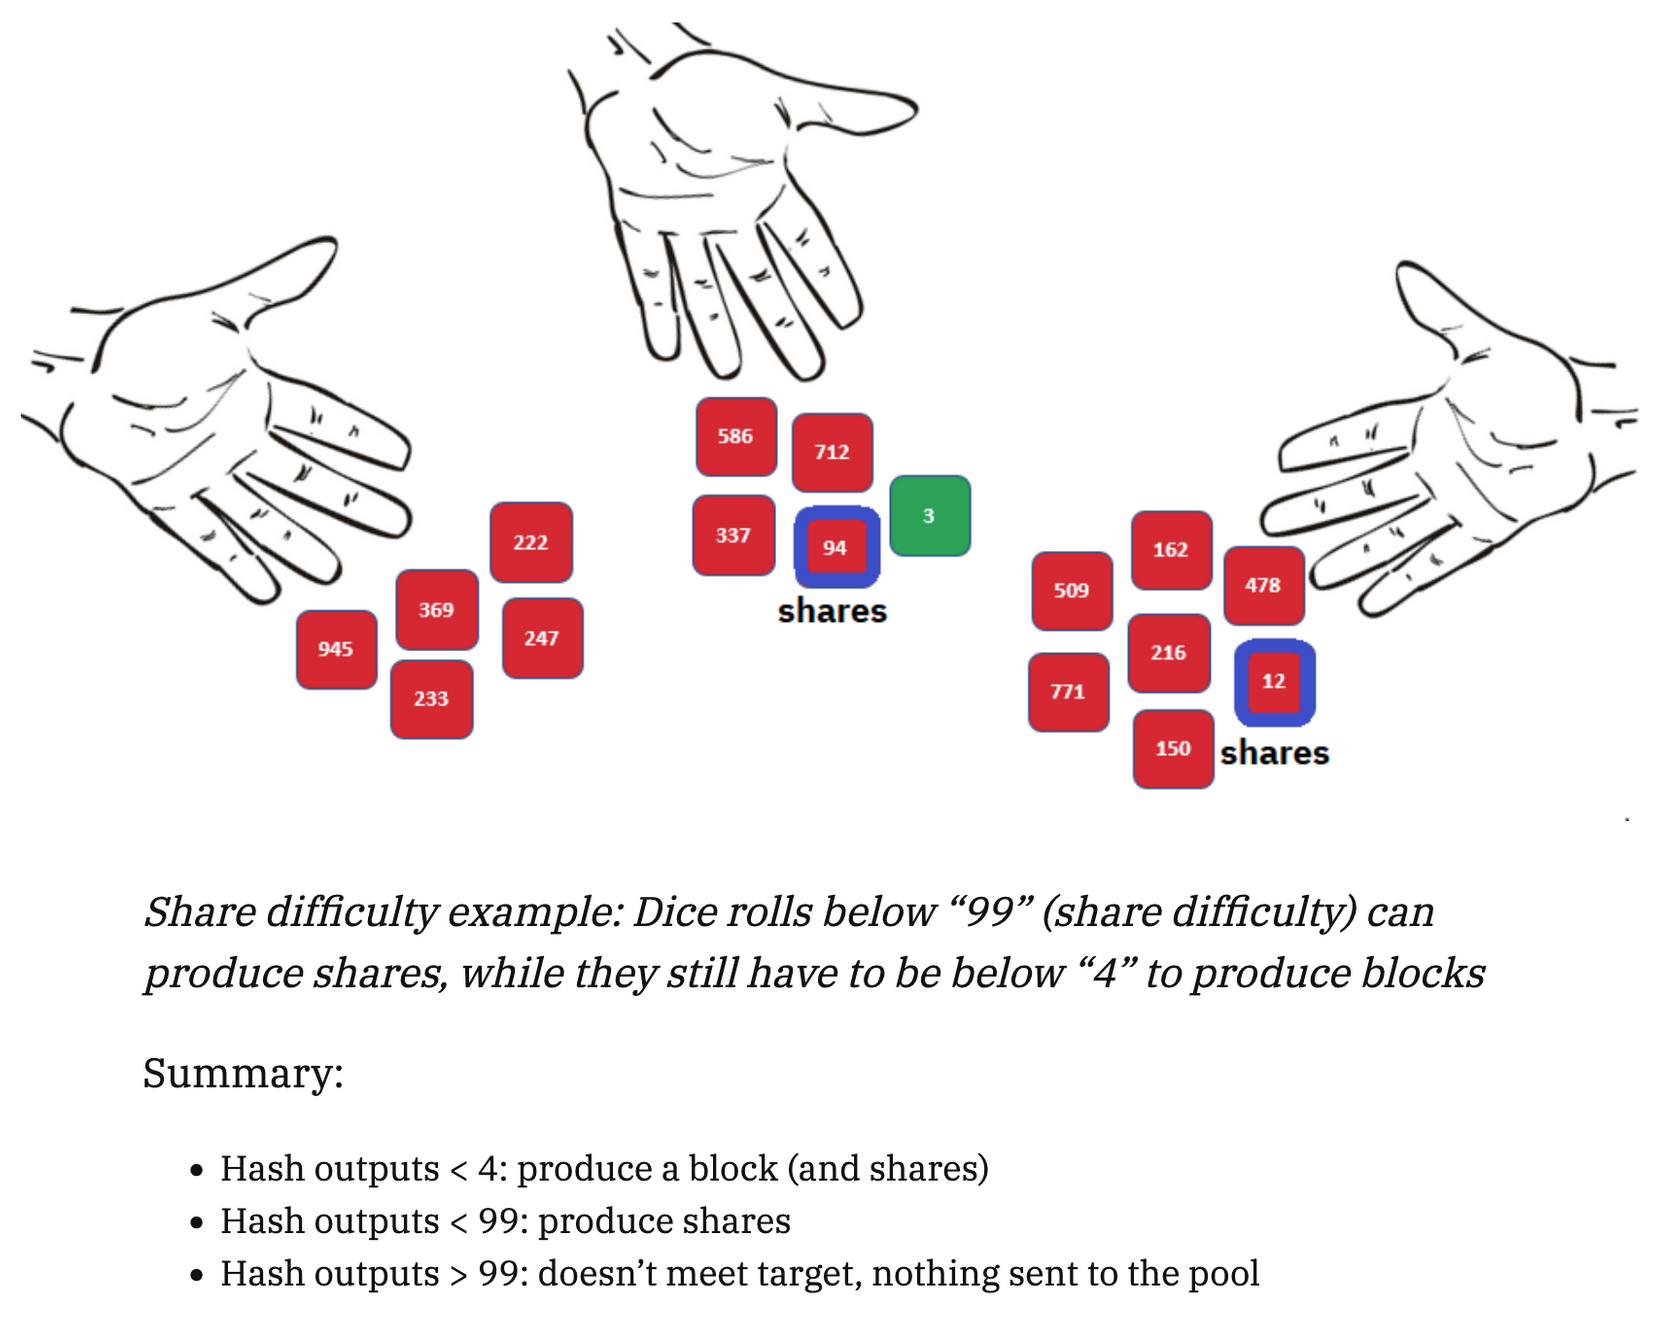
\includegraphics[width=0.65\textwidth]{Figures/mining/share.png}
\caption{Mining pool share difficulty and network difficulty \cite{bitcoinmininghandbook}}
\label{fig:mining-share}
\end{wrapfigure}
Similarly to how a solo miner has to satisfy the Bitcoin network current difficulty, in order to submit a valid block to the entire network, a miner who works in a mining pool has to find an output to the double SHA-256 function which is lower than the so called \textbf{\textit{share difficulty target}}. As represented in Figure \ref{fig:mining-share}, the mining pool sets a higher target (lower difficulty) for earning a share, typically more than 1,000 times easier than the Bitcoin network's target. When someone in the pool successfully mines a block, the reward is earned by the pool and then shared with all miners in proportion to the number of shares they contributed to the effort.\medskip

\noindent The first mining pool ever created is the so called \textit{slushpool}, born in 2010. Since those year, in fact, the need for mining pool operations were increasingly faced, to reduce the above-mentioned reward variance associated with the solo mining approach. However, in order to manage all the communications between individual miners and mining pool servers, some kind of specialized pooled mining protocol had to be developed.\\
The scope of the entire next chapter is about the history and the evolution of the pooled mining protocols, which began with the so called \textit{Getwork} protocol. It contains a deep exploration of these protocols from an operational point of view, underlining the differences between them, with their relative pros and cons.
